\cotefile{29}
\scanpage{63}\mspage{3.}
d'application \unsure{ds|dans} le théorème de spécialisation \deleted{\unsure{du groupe|des groupes}} des variétés \unsure{lisses} ---

Lorsque $X$ n'est pas \unsure{normale|normal}, on utilise la descente ---- À détailler.

% Sketch in the left margin of the preceding lines.
\figure{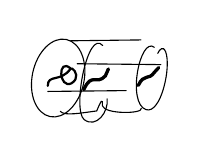
\begin{tikzpicture}[x=.55cm,y=.55cm,line cap=round]
\draw[rotate around={-12:(.62,.05)}] (.62,.05) ellipse (.60 and .91);
\draw[thin] (1.65,.80) .. controls (1.30,1.20) and (.94,-.68) .. (1.22,-.91) .. controls (1.50,-1.12) and (1.79,-.73) .. (1.75,-.43);
\draw (2.84,.76) .. controls (2.51,1.02) and (2.20,-.53) .. (2.65,-.68) .. controls (2.99,-.79) and (3.24,.31) .. (3.10,.66) .. controls (3.04,.80) and (2.96,.71) .. (2.92,.62);
\draw (.91,.91)--(2.53,.93) (1.06,.38)--(2.99,.36) (.38,-.26)--(2.19,-.24);
\draw (.67,-.72) .. controls (.77,-.83) and (1.12,-.76) .. (1.51,-.71) .. controls (1.61,-.47) and (1.65,-.40) .. (1.64,-.59) .. controls (1.69,-.79) and (2.58,-.78) .. (2.54,-.65);
\draw[thick] (.38,-.13).. controls (.38,.15) and (.68,-.06) .. (.91,.27) .. controls (.60,.54) and (.63,-.22) .. (.93,-.07) .. controls (1.11,.04) and (1.03,.22) .. (.94,.27);
\draw[very thick] (1.21,-.22).. controls (1.40,.20) and (1.50,-.13) .. (1.71,.10) --(1.78,.26);
\draw[very thick] (2.47,-.12).. controls (2.60,.16) and (2.71,-.01) .. (2.84,.18)--(2.94,.29);
\end{tikzpicture}}

% Vertical emphasis stroke beside this corollary.
\uline{Corollaire} \deleted{\illegible{1}} Soit $U$ de type fini sur $k$, $Y$
\deleted{\unsure{de type fini sur}} \unsure{propre.|propr.} sur $k$ \inserted{$y\in Y$} $R$ un revêt
étale \inserted{\unsure{gal|soit}} de $U\times_k Y$, de \unsure{groupe|gp} \unsure{$\Gamma$|$\pi$} premier \unsure{à $p$}.
\deleted{\unsure{Alors $U$}} Si $R_y$ est un rev. fini trivial,
Alors $R$ est, au dessus d'un voisinage \deleted{\unsure{de $U\times_k y$}}
$y$, l'image inverse d'un rev. \unsure{étale} d'un tel voisinage.

% Two vertical emphasis strokes beside this corollary.
\uline{Cor.} Soient $X'$, $X''$ propres sur $k$,
$Z'$ ($Z''$) des parties fermées, \deleted{\unsure{alors}} considérons
\deleted{\unsure{$Z$}} $X=\unsure{{\alpha}'|X'}\times{\alpha}''$, $Z=Z'\times X''\cup X'\times Z''$, enfin considérons
les groupes $\pi_1^t(X';Z',x')$, $\pi_1^t(X'';Z'';x'')$ et
$\pi_1^t(X\deleted{\unsure{'\times X''}};Z,x)$, \deleted{Alors} \unsure{soit|notés} $\pi,\pi';\pi''$. Alors
\[
\deleted{\pi_1^t(X)}\;\pi\longrightarrow\pi'\times\pi''
\]
est un \uline{isomorphisme}.

% Two vertical emphasis strokes beside this corollary.
\uline{Cor.} Soient $X$ $Y$ de type fini sur $k$. Considérons
$\pi'_1(X)$ \unsure{et,|et} $\pi'_1(Y)$, \inserted{$\pi'_1(X\times Y)$} [rev. étls premiers à la car].
Alors $\pi'_1(X\times Y)\simeq\pi'_1(X)\times\pi'_1(Y)$.
% archive sheet number: 62
\scanpage{64}\mspage{4.}
% Long bracket beside the initial setup.
\diagram{\begin{tikzcd}[ampersand replacement=\&,column sep=small,row sep=small]
\& X'\ \text{normalisé}\arrow[d] \& {}\\
Y\subset \& X\text{ -- }\underset{\text{\unsure{réduit|réduite}}}{\text{\uline{\unsure{complète|complet}}}} \& U=X-Y
\end{tikzcd}}

$Y_1$ -- $Y_r$ les composantes de $Y$ de codim $1$ ds $X$

$Y'_{ij}$ les images inverses des $Y_i$ ds $X'$

\deleted{\unsure{$\pi'_1$}\ \uline{Th} (?) $\pi_1(U)$ \inserted{le quotient de $\pi_1(U)$ par le} le noyau de $\pi_1(U)\to\pi_1(X)$
est \unsure{son sous-groupe|un sous-groupe} de} Considérons les rev. étales de $X-Y$ qui
\deleted{\unsure{sont de t. fini|se définissent|sont classifiés}} donnent des rev. \uuline{doux} des $\underline{O}_{y_{ij}}$,
ils sont classifiés par un groupe de type galoisien $\pi$.

\uline{\unsure{Thm.|Th.}} Le groupe $\pi$ est top. de génération finie.

\uline{Cor. 1} Soit $X$ complète, $Y$ de codim $\geq 2$, \inserted{$U=X-Y$.} Alors $\pi_1(\unsure{U|X}\deleted{\unsure{-Y}})$
est top. de présentation finie

\uline{Cor 2} Soit $X$ \deleted{de type} rég. Alors $\pi'_1(X)$ est top. de
type fini
% Two short horizontal ruling strokes below the text. Faint offset strokes across the lower half.
% archive sheet number: 63
\scanpage{65}
\[
\pi_1(X\times Y)\xrightarrow{\underline{\mathrm{surj}}}\pi_1(X)\times\pi_1(Y)
\]

\diagram{\begin{tikzcd}[ampersand replacement=\&,column sep=small]
X\arrow[d]\&[-1em]\supset Z\\
Y\&{}
\end{tikzcd}}

\[
\pi_1(Z)\unsure{\longrightarrow|-}\pi_1(X)\unsure{\longrightarrow|-}\pi_1(Y)
\]

\diagram{\begin{tikzcd}[ampersand replacement=\&,row sep=small]
X''\arrow[d,shift left=.6ex]\arrow[d,shift right=.6ex]\\
X'\arrow[d]\\
X\arrow[d]\\
\cdot
\end{tikzcd}}

\figure{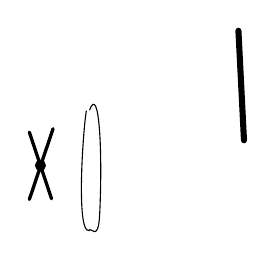
\begin{tikzpicture}[x=.47cm,y=.47cm,line cap=round]
\draw[very thick] (-.3,.9)--(.3,-.9) (-.3,-.92)--(.34,.99);
\fill (0,0) circle (.15);
\draw (1.33,1.50) .. controls (1.60,2.22) and (1.68,.26) .. (1.60,-1.33) .. controls (1.56,-2.11) and (1.36,-1.63) .. (1.31,-1.76) .. controls (.96,-1.82) and (1.15,.96) .. (1.24,1.47);
\draw[line width=2.2pt] (5.35,3.64)--(5.50,.68);
\end{tikzpicture}}

\diagram{\begin{tikzcd}[ampersand replacement=\&,column sep=small,row sep=0pt]
X\&\subset\&\widehat X\&\text{\unsure{normaux}}\\
\rotatebox{90}{$\subset$}\&{}\&\rotatebox{90}{$\subset$}\&{}\\
X_0\&\subset\&\deleted{\unsure{X}}\widehat X_0\&\text{pts singuliers}
\end{tikzcd}}

\figure{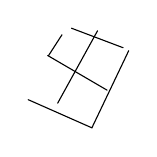
\begin{tikzpicture}[x=.55cm,y=.55cm,line cap=round]
\draw (-.77,.48)--(-.46,.96) (-.79,.48)--(.58,-.32) (-.24,1.11)--(.95,.66);
\draw (.36,1.05)--(-.56,-.62) (1.08,.59)--(.23,-1.19)--(-1.24,-.54);
\end{tikzpicture}}

\diagram{\begin{tikzcd}[ampersand replacement=\&,column sep=small,row sep=small]
Y'\arrow[r,dash]\arrow[d]\&X'\arrow[d]\\
Y\&[-.5em]{}\llap{$\subset\;$}X\arrow[d]\\
{}\&P^{r}
\end{tikzcd}}

\diagram{\begin{tikzcd}[ampersand replacement=\&,column sep=small,row sep=small]
X'\arrow[d]\&\subset\&\overline{X}'\arrow[d]\\
X\arrow[d]\&\subset\&\overline X\arrow[dll]\\
P^r\&{}\&{}
\end{tikzcd}}

\diagram{\begin{tikzcd}[ampersand replacement=\&,column sep=small,row sep=small]
Y\arrow[r]\arrow[d]\&X\arrow[d]\\
H\arrow[r]\&P^r\\[-.75em]
/K\&/k
\end{tikzcd}}

\[
\pi_1(Y)\longrightarrow\pi_1(X)
\]
$X$ normal

\[
\pi_1(Y')\xrightarrow{\mathrm{surj}??}\pi_1(X)
\]

\[
\pi_1(X)
\]

\figure{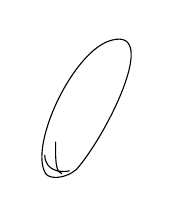
\begin{tikzpicture}[x=.60cm,y=.60cm,line cap=round]
\draw (.06,.06) .. controls (-.31,.65) and (.66,2.71) .. (1.47,2.89) .. controls (2.46,3.14) and (1.38,.92) .. (.71,.15) .. controls (.47,-.05) and (.15,-.06) .. (.06,.06);
\draw (.04,.45) .. controls (.05,.12) and (.37,.08) .. (.56,.12) (.27,.73) .. controls (.26,.20) and (.30,.10) .. (.40,.06);
\end{tikzpicture}}

\[
\deleted{\pi_1(Y)\to\pi_1(X)\leftarrow\pi_1(X-Y)}
\]
% archive sheet number: 64
\scanpage{66}\mspage{A.}
\margin{\uline{$\pi_1$ birationnel}}
% slanted
\uline{Th.} Soient $k$ un corps alg. clos, $X$ schéma \deleted{propre}\inserted{connexe}
sur $k$, \deleted{$Y$ une partie fermée} tel que tte
composante irréductible $X_i$ soit isomorphe (pour
la structure réduite induite) au \deleted{\unsure{la en question|la complémentaire}}
complémentaire d'une partie fermée de
codim $\geq 2$ dans un schéma propre sur $k$.
\margin{\uline{Question} Soit $Y\subset X$ fermé, de codim $\geq 2$, alors $\pi_1(X-Y)\to\pi_1(X)$ a un noyau de type fini???}
% slanted
Alors $\pi_1(X)$ est top. de type fini.

Démonstration. Par SGA IX 6.2, on est
ramené au cas où $X$ est \deleted{\uline{irréductible}}\inserted{intègre}, \deleted{de}\inserted{et} de
la forme $X=Z-Y$, où $Z$ est propre et $Y$ de
codim $\geq 2$ dans $Z$. On aura \unsure{aussi|ainsi},
$X=\overline X-\overline X\cap Y$, et $\overline X$ étant une composante irréductible de $Z$, $\overline X\cap Y$ y est \unsure{en|de} codim $\geq 2$. Donc
on peut supposer $Z$ \deleted{\unsure{irréductible|réduit}}\inserted{intègre}, et on est
ramené à prouver le

\uline{Corollaire} $\deleted{\unsure{X}}Z$ intègre et propre sur $k$, $Y$ \inserted{fermé} de
codim $\geq 2$ dans $Z$, $X=Z-Y$, alors $\pi_1(X)$ est
top de type fini.

Soit $Z'\to Z$ un morphisme propre
surjectif, avec $Z'$ intègre, soit $X'$ l'image
inverse de $X$ dans $Z'$, \deleted{\unsure{on|soit}} $X'=Z'-Y'$, et
$Y'$ de codim $\geq 2$ \inserted{ds $Z'$}. Par loc cit. il
suffit de prouver que $\pi_1(X')$ est top.$^{\mathrm t}$
de type fini. Par le \uline{lemme de Chow},
% archive sheet number: 65
\scanpage{67}\mspage{B.}
on peut donc supposer que
$Z$ est \uline{projectif}, \deleted{Si $\dim$} et $=$ \uline{normal}
si on veut. Si \inserted{$\dim Z\leq 0$, trivial. Si} $\dim Z=1$, on aura $Y=\varnothing$,
i.e. $X=Z$, et le th. est connu. Si $\dim Z\geq 2$
on utilise ceci :

\uline{Lemme} de \uline{Bertini} : (Zariski) Soit $k$ corps,
$X\xrightarrow{f}P^r_k$ un \uline{morphisme}, avec $X$ \deleted{\unsure{intègre}}\inserted{irréductible},
$\dim f(X)=n$, soit $1\leq\unsure{s|5}\leq\unsure{n|r}-1$, \deleted{et} soit
$u$ \deleted{le} point générique de $\underbrace{P^r_k\times\cdots\times P^r_k}_{s}$, et
$K$ une clôture algébrique de $k(u)$, enfin
$L_u$ la variété linéaire dans $P^r_K$ définie
par $u$, et $X_u=X\times_{P^r_k}L_u=X_K\times_{P^r_K} L_u$.
\margin{peut-on remplacer ``irréductible'' par ``connexe'' ? \uline{non}}
% slanted
Alors $X_u$ est irréductible.

% Diagram in the left margin, spanning the lemma and corollary.
\diagram{\begin{tikzcd}[ampersand replacement=\&,row sep=small,column sep=small]
X'_u\arrow[d]\&{}\&X'\arrow[d]\\
X_u\arrow[r]\arrow[d]\&X_K\arrow[r]\arrow[d]\&X\arrow[d]\\
L_u\arrow[r]\&P^r_K\arrow[r]\&P^r_k
\end{tikzcd}}

\uline{Corollaire} \deleted{\unsure{$\pi_1(X)$|Il est}} Si $X$ est \uline{normal},
alors $\pi_1(X_u)\to\pi_1(X)$ est \uline{surjectif}.

En effet, si $X'$ est un revêtement \deleted{\unsure{normal|connexe}}
étale connexe de $X$, étant normal il est
\uline{irréductible}, donc $X'_u=X'\times_X X_u$ est
irréductible, donc connexe, OK.
\margin{Si on admet le th. de connexion, on \deleted{peut} \deleted{\unsure{peut}} \unsure{aussi} utiliser une section \deleted{\unsure{plus|fibrée}} ``spéciale'' ..... p. ex une courbe ...}
% slanted
% archive sheet number: 66
\scanpage{68}\mspage{C}
Reprenons alors $Z$ normal de dim $n\geq 2$, et
$X=Z-Y$. Plongeons $Z$ dans $P^r$, et le morphisme
induit $f:X\to P^r$. On prend $s=n-1$, de
sorte que $X_u$ \deleted{est une \uline{courbe}} \inserted{$=X_K\cap L_u=Z_K\cap L_u$ \deleted{\unsure{$=$}}, car $Y_K\cap L_u=\varnothing$,}
donc $X_u=Z_K\cap L_u$ est une \uline{courbe} \deleted{de
genre $g$} projective, d'ailleurs normale. Si $g$
est son genre, il résulte alors du corollaire
au lemme de Bertini que $\pi_1(X)$ admet
$2g$ générateurs topologiques, OK.

\uline{Conséquence}. Soit $K$ une extension
de type fini d'un corps $k$. Il
existe tjrs des modèles projectifs,
\deleted{\unsure{(donc|celui-ci} \unsure{normaux|normal}} à fortiori propres, et
normaux si on veut, \deleted{\unsure{donc|et} réguliers en
codim $\leq 1$, \inserted{Soit $X$ \unsure{de}} \unsure{la variété de|le modèle de} \unsure{des|du}
modèles \uline{réguliers} $U$ qui sont \deleted{\unsure{qui}}
\deleted{\unsure{par}} ``\uline{presque propres}'', i.e. complémentaires
d'un ens fermé de codim $\geq 2$ dans
un modèle propre $X$. D'ailleurs, \unsure{tous|ts|ttes} les
modèles $U$ comme dessus, \unsure{ordonnés|ordonnées} par}
% Small fork in the left margin of the cancelled paragraph.
\diagram{\begin{tikzcd}[ampersand replacement=\&,row sep=small,column sep=small]
{}\&X''\arrow[dl,dash]\arrow[dr,dash]\&{}\\
X\&{}\&X'
\end{tikzcd}}
% archive sheet number: 67
\scanpage{69}\mspage{D}
D'ailleurs les modèles propres et normaux, pour la
\deleted{la} relation de domination, forment un
ordonné \uline{filtrant croissant}. \deleted{\unsure{On se}} Soit $U$
un \deleted{\unsure{les|tel}} modèle \inserted{régulier de $K$} \deleted{\unsure{tel l'ensemble} de ses pts
réguliers}, et soit $X_{\unsure{1|0|u}}$ \deleted{\unsure{dominé de} $X_0$} \inserted{propre \deleted{\unsure{normal}} et \uline{normal}}.

% At the upper left, three labels and an abandoned connection.
\diagram{\begin{tikzcd}[ampersand replacement=\&,row sep=small,column sep=small]
{}\&X''\arrow[dl,dash]\&{}\\
\deleted{\unsure{U}}X\arrow[rr,dash]\&{}\&X'\deleted{\unsure{X'}}
\end{tikzcd}}

\deleted{Soit $U_0$ l'ens des pts de $U_0$ où
l'application rationnelle évidente \deleted{\unsure{$X$}}
$U_0\to X_1$ induit \deleted{\unsure{un $g$}} est
définie, c'est \inserted{le compl. de \unsure{l'ens|celui} d'} \deleted{un} un fermé
codim $\geq 2$, \deleted{\unsure{donc d'où le}}
et on a donc
\deleted{complémentaire dans $X_0$ d'un ens
fermé de codim $\geq 2$.} On a un \deleted{hom
canonique}, diagramme commutatif,
d'où on voit qu'on a
un hom surjectif}

\diagram{\begin{tikzcd}[ampersand replacement=\&,column sep=small,row sep=small]
X_{\unsure{1}}\arrow[d,"f"]\&{}\&{}\\
X_0\&{}\llap{$\underset{i}{\supset}\;$}U\&{}\llap{$\underset{j}{\supset}\;$}U_{0}\arrow[ull,"g"']
\end{tikzcd}}

\diagram{\begin{tikzcd}[ampersand replacement=\&,column sep=small,row sep=small]
\pi_1(X_1)\arrow[d,"f_*"]\&{}\&\deleted{\pi_1(U_1)}\arrow[ll]\\
\pi_1(X_0)\&\pi_1(U_0)\arrow[l]\&\pi_1(U_1)\arrow[l,"\sim" ,"\substack{\text{th.}\\\text{de pureté}}"' ]\arrow[ull,"g_*"']
\end{tikzcd}}

L'application rationnelle évidente
$U\to X$ étant définie dans
le complémentaire d'une partie fermée de
codim $\geq 2$, on voit que (par le th. de
pureté) on a un hom \uline{surjectif} (car $X$ \unsure{norm.?|normal}]
\[
\pi_1(U)\to\pi_1(X)
\]
d'où à la limite un \uline{hom \uline{surjectif}}
\[
\pi_1\unsure{U;\Omega)|(U;\Omega)|(U,\Omega)}\longrightarrow
\varprojlim_{\substack{X\ \text{modèle}\\\text{propre}}}\pi_1(X;\Omega)
\]
où $\Omega$ est une extension alg. close de $K$.
\margin{\deleted{\unsure{cf}}}
% slanted
% archive sheet number: 68
\scanpage{70}\mspage{E.}
Le deuxième est est appelé le \uline{groupe fondamental
birationnel} de $K/k$. [N.B. il y aurait
\unsure{à} l'introduire plutôt comme groupe alg.
sur $K$], \inserted{noté $\pi_1(K/k;\Omega)$. Pour tt modèle \uline{propre} \uline{projectif} $X$, $\pi_1(X;\Omega)$ est un quotient de $\pi_1(K/k)$.} On voit donc qu'il est \unsure{isomorphe|toujours}
\unsure{à un|un} quotient de $\pi_1(U)$. Donc, comme
$U$ peut être pris complémentaire d'une partie fermée
de codim $\geq 2$ ds un \unsure{schéma|sch.} intègre propre :

\uline{Th.} Si $K/k$ est une extension de
type fini, avec $k$ alg. clos, alors
\deleted{\illegible{1}} $\pi_1(K/k;\Omega)$ est top.$^{\mathrm t}$ de type fini.

\margin{\uline{Remarque} Si $K$ a un modèle propre régulier $X$, alors pour $X'$ \deleted{propre} normal dominant $X$, on a $\pi_1(X';\Omega)\overset{\sim}{\longrightarrow}\pi_1(X;\Omega)$, donc le système projectif des $\pi_1(X';\Omega)$, $X'$ propre normal, est essentiellement constant. Qu'en est-il en général ??? Si $X$ est un modèle propre normal, \deleted{\unsure{tout}} $U$ l'ens de ses pts réguliers, est-il vrai que $\pi_1(U;\Omega)\to\pi_1(K/k;\Omega)$ est bijectif, i.e. que tte \deleted{\unsure{variété $X$}} \unsure{extension} finie $K'$ de $K$, non ramifiée sur $U$, est non ramifiée sur un modèle \inserted{\unsure{normal}} $X'$ \unsure{dérivant de|distinct de|dominant} $X$ pour \unsure{certains|certain} \unsure{$X'$|$X$} ? C'est une question en fait de schémas généraux ....}
% slanted
% archive sheet number: 69
\scanpage{71}\mspage{F.}
\margin{\uline{Pic birationnel}}
% slanted
\uline{Théorème} Soient $f:X\to Y$ un morphisme \inserted{birationnel} dominant
de préschémas intègres normaux, \deleted{et} propres sur $k$,
avec $Y$ \deleted{loc. \uline{factoriel}}\inserted{\uline{régulier}}. Alors le morphisme
\[
\underline{\mathrm{Pic}}^{\tau}_Y\longrightarrow\underline{\mathrm{Pic}}^{\tau}_X
\]
est un \uline{isomorphisme}.
\margin{$X$ normal ``sur $k$'' ?}
% slanted
\margin{\unsure{faut-il|peut-on} $=$ \deleted{\unsure{supposer}} $Y$ \deleted{régulier ??} \deleted{\unsure{non}} \unsure{simple|sing.} sur $k$ ?}
% slanted
\margin{N.B. factoriel ne suffit pas $=$ du pt de \unsure{vue} \unsure{ensembliste|ensemblips}, cf cônes ---}
% slanted

C'est un \uline{monomorphisme} grâce au fait que
$f_*(\underline{O}_X)=\underline{O}_Y$ (universellement sur $k$ !), donc une
immersion fermée puisque un hom de groupes
-- ou \unsure{parce que} propre. Montrons que c'est
\uline{surjectif}. Soit $U$ l'ouvert de $Y$ où $f^{-1}$ est
défini, comme $Y$ est factoriel, on a
$\mathrm{Pic}(X)\overset{\sim}{\longrightarrow}\mathrm{Pic}(U)$, d'où, utilisant
\diagram{\begin{tikzcd}[ampersand replacement=\&,column sep=small,row sep=small]
{}\&X\arrow[d,"f"]\\
U\arrow[ur,"g"]\arrow[r,"i"]\&Y
\end{tikzcd}}
, le diagramme commutatif
\diagram{\begin{tikzcd}[ampersand replacement=\&,column sep=small,row sep=small]
{}\&\mathrm{Pic}(X)\arrow[dl,leftrightarrow,"g^*"]\\
\mathrm{Pic}(U)\&\mathrm{Pic}(Y)\arrow[l,"i^*","\sim"']\arrow[u,"f^*"']
\end{tikzcd}}
qui montre que $\mathrm{Pic}(Y)\to\mathrm{Pic}(X)$ est un hom
sur un facteur direct, l'image étant \unsure{formé|formée} des
$\xi$ telles que $\deleted{\unsure{g^*(\xi)=0.|f^*(\xi)=0}}\ \xi=f^*i^{*-1}g^*(\xi)$. Or
$\xi$ est \deleted{\unsure{num}} $\tau$-équivalente à $0$, \inserted{donc $\exists\,\unsure{n|m}\xi$ est alg$^{\mathrm t}$ équiv. à $0$,} \deleted{\unsure{son}} $g^*(\xi)$
\deleted{est} \deleted{$\tau$-équivalent}\inserted{alg. équiv.} à $0$, donc $i^{*-1}g^*(\xi)$ \deleted{\unsure{est}} aussi,
donc \deleted{\unsure{$n$}} $f^*i^{*-1}g^*(\xi)$ \inserted{$=n f^*(i^{*-1}g^*(\xi))$} \unsure{égal$^{\mathrm t}$}. D'autre part, on voit que
$\xi-f^*i^{*-1}\deleted{g^*(\xi)}$ \deleted{\unsure{est diviseur représenté il}} est représenté par un
\margin{\unsure{Revenir au dessin|Revenir au discours|Raisonner en termes} des cycles !}
% slanted
\margin{$Y$ \unsure{régulier|séparation} ?? ou \unsure{simple|tjrs simple} sur $k$}
% slanted
% archive sheet number: 70
\scanpage{72}\mspage{G.}
diviseur $\sum n_i X_i$, où les $X_i$ sont les ``diviseurs
singuliers'' pour $f$. Il reste donc à voir que si
une telle combinaison linéaire est \deleted{\unsure{algébriquement}}
$\tau$-équivalente à $0$, elle est nulle. \deleted{\unsure{\illegible{1}|Ce}} C'est là
un lemme bien connu ----
\margin{vérifier ? On peut se ramener au cas projectif}
% slanted

Ainsi, $f^*:\underline{\mathrm{Pic}}^\tau_Y\to\underline{\mathrm{Pic}}^\tau_X$ est une \uline{immersion
surjective}. Il \uline{reste à prouver} qu'elle induit
un isom sur les espaces tangents à l'origine,
donc à vérifier le
\margin{\uline{insuffisant}}
% slanted

\uline{Corollaire} Sous les conditions du th., \unsure{le l'homomorphisme|l'homomorphisme}
\[
f^*:H^1(Y,\underline{O}_Y)\to H^1(X,\underline{O}_X)
\]
est un isomorphisme.

On sait déjà que c'est injectif, la question
est la surjectivité. \deleted{Il suffit} En caractéristique $p>0$,
il suffit de prouver qu'on a \unsure{bijectivité}
\[
\begin{aligned}
H^1(Y,\underline{O}_Y)^F&\longrightarrow H^1(X,\underline{O}_X)^F\\
{}_{F^{\unsure{\nu|v}}}H^1(Y,\underline{O}_Y)&\unsure{\longrightarrow|-}{}_{F^{\nu}}H^1(X,\underline{O}_X)
\end{aligned}
\]
où $F$ est le Frobenius. Le premier
hom s'écrit
\[
H^1(Y,\mathbb Z/p\mathbb Z)\to H^1(X,\mathbb Z/p\mathbb Z)
\]
% archive sheet number: 71
\scanpage{73}\mspage{H}\deleted{\unsure{H}}
c'est un isomorphisme à cause du fait que
$\pi_1(X)\unsure{\to|-}\pi_1(Y)$ est un isomorphisme [grâce au
th. de pureté sur $Y$]
\margin{$Y$ \uline{régulier} \unsure{$[$|$\Gamma$}}
% slanted

Le deuxième homomorphisme s'écrit
\[
H^0(Y,\underline{O}_Y/\underline{O}_Y^{p^{\unsure{\nu|v}}})\to H^0(X,\underline{O}_X/\underline{O}_X^{p^\nu})
\]
[grâce au fait que $X$, $Y$ sont réduits],
ou aussi, supposant que $k$ est alg. clos
donc parfait, s'interprète comme
\margin{$Y$ \unsure{simple|intègre} sur $k$ (?)}
% slanted
\[
f^*:H^0(Y,\underline{O}_Y^{p^{-\nu}}/\underline{O}_Y)\to H^0(X,\underline{O}_X^{p^{-\nu}}/\underline{O}_X)
\]

Ce dernier est bijectif grâce à la
\uline{normalité} de $X$ et $Y$, car \deleted{\unsure{si $f$}} avec
les notations ci-dessus, on a un
diagramme commutatif
\diagram{\begin{tikzcd}[ampersand replacement=\&,column sep=large,row sep=small]
{}\&T(X)\arrow[dl,"g^*"]\\
T(U)\&T(Y)\arrow[l,"i^*","\sim"']\arrow[u,"f^*"']
\end{tikzcd}}
avec $g^*$ \uline{injective} [car $\underline{O}_X^{p^{-\nu}}/\underline{O}_X^{\unsure{?|2}}$ est \deleted{\unsure{l'}} 
\uline{sans torsion} ---], donc $f^*$ et $i^{*-1}g^*$ sont des isom
inverses l'un de l'autre.
\margin{$X$ \uline{\unsure{normale|normal ?|normal}}}
% slanted
% archive sheet number: 72
\scanpage{74}\mspage{I}
Dans le cas où $k$ est de car. $0$, on
peut supposer que $k$ est \deleted{de type fini
sur \unsure{$\mathbb Q$}}, le corps \unsure{des|de} fonctions d'un
schéma intègre $S$ de type fini sur $\mathbb Z$,
et que $f:X\unsure{-|\to}\unsure{Y|X}$ provient d'un
morphisme de $S$-préschémas $\bar f:\overline X\to\overline Y$,
intègres, $\overline Y$ simple sur $S$, et $\overline X$ \deleted{simple}
normal sur $S$, les fibres de l'un et
l'autre étant univ.$^{\mathrm t}$ connexes. \deleted{Alors pour
\unsure{tt|$\forall$} $y\in Y$, \unsure{s.c.|si} \unsure{$\mathrm{Ker}$} $H^1(\unsure{Y|X},\underline{O}_Y)\to H^1(X,\underline{O}_X)$
est de dim $r$, il existe un} on
\deleted{peut supposer qu'il existe un} On peut
supposer aussi $X$ et $Y$ coh. plats sur
$S$ en dim $1$, \deleted{enfin que} alors
\deleted{\unsure{cette}} \unsure{Ker|l'hom} $R^1\unsure{q_*|p_*}(\underline{O}_{\overline Y})\unsure{-|\to} R^1p_*(\underline{O}_{\overline X})$ est injectif,
\deleted{et que} (car il l'est en tt pt
par \unsure{ci-dessus dit|ci dessus dit}) alors \unsure{restreignant} $S$, si
le \unsure{conoyau|corang} de $H^1(Y,\underline{O}_Y)\unsure{-|\to}H^1(X,\underline{O}_X)$
est de dim $r$, la $=$ chose sera
vraie pour les fibres en \uline{tous} les \unsure{pts} \deleted{\unsure{de}}
$s\in S$, en particulier en \unsure{aux|des|au} pts de
% archive sheet number: 73
\scanpage{75}\mspage{J}
car $>0$. Cela prouve $r=0$, et achève la
démonstration.

\uline{Corollaire} 1 Invariance birationnelle de $\underline{\mathrm{Pic}}^\tau_{X/k}$
pour $X$ propre et simple sur $k$.

\uline{Corollaire} 2 Soit $K$ une extension
\deleted{régulière}\inserted{séparable primaire} de type fini de $k$, admettant
un modèle \deleted{régulier \unsure{et}} propre et \uline{simple}
sur $k$. Alors $\varinjlim_X\underline{\mathrm{Pic}}^\tau_{X/k}$, où $X$ parcourt
les Modèles propres et normaux \inserted{``sur'' $k$} de $K$
existe au sens \unsure{trivial|strict} [le système \deleted{projectif}\inserted{inductif}
est essentiellement constant]
\margin{\uline{N.B.} Si $k$ n'est pas parfait, et $K$ est de dim $1$ sur $k$, \deleted{\unsure{sur}} c'est une \unsure{restriction|condition} un peu idiote !.}
% slanted

\uline{Question}. Le cor. 2 reste-t-il valable
en supposant seulement que $K$ admette
un modèle ``normal sur $k$'' ?? \deleted{Il y aurait} \deleted{\unsure{On}}\inserted{\unsure{Cela|Ceci|Car|le cas}}
\deleted{du moins} équivaudrait à la conjonction des
assertions suivantes

(i) $\dim\underline{\mathrm{Pic}}_{X/k}$ reste majoré

(ii) ordre $\mathrm{Tors}\,\underline{\mathrm{Pic}}(X/k)$ reste majoré

(iii) $\dim H^1(X,\underline{O}_X)$ reste majoré.
% Tors Pic and the H^1 expression in the last two lines are individually encircled.
\margin{N.B. (i) résulte de (iii)}
% archive sheet number: 74
\scanpage{76}\mspage{K}
\uline{Théorème} Soit $K$ une extension de type fini du
corps $k$, \deleted{[ayant au moins un modèle
propre \inserted{\unsure{int.}} et universellement normal sur $k$]} \deleted{Soit} Il
\deleted{$(X_i)_{i\in\unsure{I|+}}$ le système ind} existe un entier $n(K/k)$
tel que pour \deleted{tout} modèle \inserted{$X$ de $K$} propre sur $k$, et
normal sur $\unsure{k|K}$, \deleted{\unsure{pour}} on ait \deleted{$\dim\underline{\mathrm{Pic}}_X$}
\[
\dim\underline{\mathrm{Pic}}_{X/k}\leq n(K/k)
\]

Démonstration. \deleted{On est ramené au cas} \inserted{S'il n'existe pas de}
modèle $X$ du type indiqué, c'est trivial.
Sinon, $K$ est séparable sur $k$, et
$\overline K=K\otimes_k\bar k$ est une extension de type
fini du corps alg. clos $\unsure{\bar K|\bar k}$, et on
est ramené au cas où $\bar k$ est alg. clos.
On a alors
\[
\begin{aligned}
\dim\underline{\mathrm{Pic}}_{X/k}
&=\tfrac12\operatorname{rang}_{\mathbb Z_{\ell}}
  \bigl(\text{partie $l$-primaire}\\
&\qquad \text{de $\pi_1(X/k)$ rendu}\\
&\qquad \text{abélien}\bigr)
\end{aligned}
\]
et à ce titre, en vertu du théorème
de majoration uniforme \unsure{des|du} $\pi_1(X/k)$
% archive sheet number: 75
